\documentclass[aspectratio=169,11pt]{beamer}

% --- Theme ---
\usetheme{metropolis}
\usepackage{appendixnumberbeamer}

% --- Packages ---
\usepackage{fontspec}
\usepackage{minted}
\setminted{fontsize=\small,breaklines=true}
\usepackage{booktabs}
\usepackage{tikz}
\usepackage{fontawesome5}

% --- Colors ---
\definecolor{healthgreen}{RGB}{34,139,34}
\definecolor{alertred}{RGB}{220,53,69}
\setbeamercolor{alerted text}{fg=alertred}

% --- Metadata ---
\title{Module 2: Health data with Pandas}
\subtitle{Data analysis with Python for health specialists}
\author{Ya\'{e} Ulrich Gaba}
\institute{AIRINA Labs}
\date{2026}

\begin{document}

% ============================================================
\maketitle

% ============================================================
\begin{frame}{What is a DataFrame?}
\begin{columns}
\column{0.55\textwidth}
A DataFrame is a \alert{table}:
\begin{itemize}
  \item Rows = observations (patients, countries, time points)
  \item Columns = variables (age, diagnosis, lab values)
\end{itemize}

\vspace{6pt}
Think of it as \textbf{Excel with superpowers}: scriptable, reproducible, and capable of handling millions of rows.

\column{0.4\textwidth}
\centering
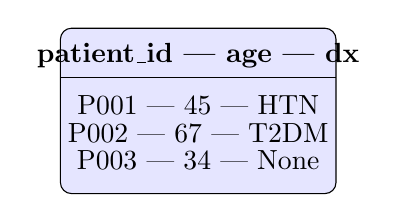
\begin{tikzpicture}[scale=0.7]
\draw[fill=blue!10, rounded corners] (0,0) rectangle (5,3);
\node at (2.5,2.5) {\textbf{patient\_id | age | dx}};
\draw (0,2.1) -- (5,2.1);
\node at (2.5,1.6) {P001 | 45 | HTN};
\node at (2.5,1.1) {P002 | 67 | T2DM};
\node at (2.5,0.6) {P003 | 34 | None};
\end{tikzpicture}
\end{columns}
\end{frame}

% ============================================================
\begin{frame}[fragile]{Creating a clinical DataFrame}
\begin{minted}{python}
import pandas as pd

data = {
    "patient_id": ["P001", "P002", "P003", "P004", "P005"],
    "age": [45, 67, 34, 52, 71],
    "sex": ["M", "F", "F", "M", "F"],
    "systolic_bp": [128, 158, 112, 145, 162],
    "hba1c": [5.4, 7.8, 5.1, 6.3, 8.2],
    "diagnosis": ["None", "T2DM", "None", "Pre-DM", "T2DM"]
}
df = pd.DataFrame(data)
df
\end{minted}
\end{frame}

% ============================================================
\begin{frame}[fragile]{Loading real health data}
\begin{minted}{python}
# CSV from a URL (Gapminder life expectancy data)
url = ("https://raw.githubusercontent.com/datasets/"
       "gapminder/main/data/gapminder.csv")
gapminder = pd.read_csv(url)
print(f"Shape: {gapminder.shape}")  # (rows, columns)

# Excel file
df = pd.read_excel("patient_records.xlsx",
                    sheet_name="Lab Results")

# WHO Global Health Observatory API
url = ("https://apps.who.int/gho/athena/api/"
       "GHO/MDG_0000000026?format=csv")
mmr = pd.read_csv(url)
\end{minted}

\begin{exampleblock}{WHO GHO}
Over 1\,000 health indicators for 194 member states. Browse at \url{https://www.who.int/data/gho/data/indicators}.
\end{exampleblock}
\end{frame}

% ============================================================
\begin{frame}[fragile]{Exploring your data}
The first thing you do with any health dataset --- \alert{before any analysis} --- is \textbf{look at it}.

\begin{minted}{python}
print(gapminder.shape)             # dimensions
print(gapminder.columns.tolist())  # column names
print(gapminder.dtypes)            # data types
gapminder.describe()               # summary statistics
gapminder.info()                   # non-null counts
\end{minted}

\vspace{4pt}
These five commands give you a complete snapshot in 30 seconds.
\end{frame}

% ============================================================
\begin{frame}[fragile]{Selecting and filtering}
\begin{minted}{python}
# Single column (Series)
ages = gapminder["lifeExp"]

# Multiple columns (DataFrame)
subset = gapminder[["country", "year", "lifeExp"]]

# Filter: diabetic patients (HbA1c >= 6.5)
diabetic = df[df["hba1c"] >= 6.5]

# Filter: African countries
africa = gapminder[gapminder["continent"] == "Africa"]

# Multiple conditions (use & and parentheses!)
high_risk = df[(df["sex"] == "F") &
               (df["age"] > 60) &
               (df["systolic_bp"] >= 140)]
\end{minted}

\begin{alertblock}{Warning}
Use \texttt{\&}, \texttt{|}, \texttt{\textasciitilde} with parentheses. Python's \texttt{and}/\texttt{or} do not work with DataFrames.
\end{alertblock}
\end{frame}

% ============================================================
\begin{frame}[fragile]{Sorting and ranking}
\begin{minted}{python}
# Countries with highest life expectancy in 2007
recent = gapminder[gapminder["year"] == 2007]
top10 = recent.sort_values("lifeExp",
                           ascending=False).head(10)
print(top10[["country", "lifeExp"]])
\end{minted}

\vspace{6pt}
\texttt{.sort\_values()} + \texttt{.head(n)} is the quick way to find the top or bottom $n$ observations.
\end{frame}

% ============================================================
\begin{frame}[fragile]{Grouping and aggregation}
\textbf{Question:} What is the average life expectancy per continent?

\begin{minted}{python}
# Single aggregation
recent.groupby("continent")["lifeExp"].mean()

# Multiple aggregations
recent.groupby("continent")["lifeExp"].agg(
    ["mean", "median", "std", "count"]
)

# Patient counts by diagnosis
df.groupby("diagnosis")["patient_id"].count()
\end{minted}

\vspace{4pt}
\texttt{.groupby()} + \texttt{.agg()} answers any \alert{``per group''} question.
\end{frame}

% ============================================================
\begin{frame}[fragile]{Creating new columns}
\begin{minted}{python}
# BMI from weight and height
df["bmi"] = df["weight_kg"] / (df["height_m"] ** 2)

# Age group (categorical from continuous)
df["age_group"] = pd.cut(
    df["age"],
    bins=[0, 18, 40, 60, 100],
    labels=["<18", "18-39", "40-59", "60+"]
)

# Binary flag
df["hypertensive"] = (df["systolic_bp"] >= 140).astype(int)
\end{minted}

\vspace{4pt}
\texttt{pd.cut()} turns a continuous variable into clinical categories --- essential for epidemiology.
\end{frame}

% ============================================================
\begin{frame}[fragile]{Saving your results}
\begin{minted}{python}
# Save to CSV (most common)
df.to_csv("cleaned_patients.csv", index=False)

# Save to Excel
df.to_excel("cleaned_patients.xlsx",
            index=False, sheet_name="Patients")
\end{minted}

\vspace{6pt}
Always save cleaned data for reproducibility. Keep the raw data untouched in a separate folder.
\end{frame}

% ============================================================
\begin{frame}{What you can do after this module}
\begin{enumerate}
  \item Load health data from CSV, Excel, or the WHO API into a DataFrame
  \item Explore any dataset in 30 seconds (\texttt{.shape}, \texttt{.describe()}, \texttt{.info()})
  \item Filter patients by clinical criteria (BP thresholds, diagnosis, age)
  \item Compute summary statistics per group (\texttt{.groupby()})
  \item Create clinical categories from continuous variables (\texttt{pd.cut()})
\end{enumerate}

\vspace{12pt}
\centering
\Large \alert{Next: Module 3 --- Data cleaning in health contexts}
\end{frame}

% ============================================================
\begin{frame}{Exercises (Hour 3)}
\begin{enumerate}
  \item \textbf{Load and explore:} Load the Gapminder dataset, display shape, dtypes, and summary statistics
  \item \textbf{Filter Africa:} Select African countries only; how many unique countries?
  \item \textbf{Decade trends:} Compute mean life expectancy by decade for Africa vs.\ Europe
  \item \textbf{Mini-project:} Build a complete WHO life expectancy analysis notebook with filtering, grouping, new columns, and a saved CSV
\end{enumerate}
\end{frame}

\end{document}
